\documentclass[twocolumn]{article}
\usepackage{mathptmx}
\usepackage[utf8]{inputenc}
\usepackage{fullpage}
\usepackage{multirow}
\usepackage[table,xcdraw]{xcolor}
\usepackage{epsfig}
\usepackage{epstopdf}
\usepackage{caption}
\usepackage{amsfonts}
\usepackage{amssymb}
\usepackage{amsmath}
\usepackage{url}
\usepackage{color}
\usepackage[colorlinks = true,
linkcolor = blue,
urlcolor  = blue,
citecolor = blue,
anchorcolor = blue]{hyperref}
\usepackage{comment}
\usepackage{graphicx}
\usepackage{cite}
\usepackage{subfigure}
\usepackage[normalem]{ulem}
\usepackage{soul}
\usepackage{array}
\newcolumntype{L}{>{\centering\arraybackslash}m{3cm}}

\date{}

\begin{document}

\title{A Flexible Machine Learning-Aware Architecture\\ for Future WLANs} 
%Machine Learning in Future WLANs: an Architectural Perspective}

\author{Francesc Wilhelmi, Sergio Barrachina-Mu\~noz, Boris Bellalta,\\ Cristina Cano, Anders Jonsson,  \& Vishnu Ram\thanks{\textit{Francesc Wilhelmi, Sergio Barrachina-Mu\~noz, Boris Bellalta, and Anders Jonsson are with Universitat Pompeu Fabra (UPF); Cristina Cano is with Universitat Oberta de Catalunya (UOC); Vishnu Ram is currently working as an independent researcher.}}}

\maketitle

\begin{abstract} 
Lots of hopes have been placed in Machine Learning (ML) as a key enabler of future wireless networks. By taking advantage of the large volumes of data generated by networks, ML is expected to deal with the ever-increasing complexity of networking problems. Unfortunately, current networking systems are not yet prepared for supporting the ensuing requirements of ML-based applications, especially for enabling procedures related to data collection, processing, and output distribution. This article points out the architectural requirements that are needed to pervasively include ML as part of future wireless networks operation. To this aim, we propose to adopt the International Telecommunications Union (ITU) unified architecture for 5G and beyond. Specifically, we look into Wireless Local Area Networks (WLANs), which, due to their nature, can be found in multiple forms, ranging from cloud-based to edge-computing-like deployments. Based on the ITU's architecture, we provide insights on the main requirements and the major challenges of introducing ML to the multiple modalities of WLANs.
\end{abstract}

% ----------------------------------
% -
% 	-- Introduction --
% -
% ----------------------------------
\section{Introduction} 
\label{section:introduction}
Wireless communications have reached a point where a paradigm shift is required for satisfying the increasing needs of next-generation applications \cite{osseiran2014scenarios}. Based on the current trend, Artificial Intelligence (AI), and more precisely Machine Learning (ML), are expected to conduct a revolution, especially regarding the network planning, operation, and management of the fifth and sixth generation (5G/6G) of mobile communications. 

ML is meant to empower a computational system for learning automatically, based on experience, so that future situations can be properly managed without having been programmed explicitly. Concerning wireless communications, there is a huge amount of unexploited data generated at both infrastructure and user levels, which could be extremely useful to ML mechanisms for learning complex patterns. According to the information extracted by these methods, network performance can be improved. For instance, the behavior of users in a given network-oriented service can be predicted through ML, based on the information from previous sessions. This information would enable to better accommodate network resources in future sessions, thus leading to an optimized solution.

Unfortunately, the potential benefits of ML solutions for real networks are currently limited by the existing infrastructure, which is not yet prepared to accommodate ML-oriented tasks such as data collection, processing, and output distribution. Instead, current networking systems are typically meant for delivering content, without taking into account the underlying characteristics of the processes that generate it. 

The first steps towards AI-enabled networking are currently being made in 5G through network function virtualization (NFV). Unlike traditional hardware-based networks, NFV allows rapid elasticity and fast reconfiguration on assigning network resources, which is particularly useful to enable verticals such as autonomous driving in the automotive sector or smart manufacturing in Industry 4.0. Besides, network virtualization is useful to boost inter-operator coordination, which would bring the ML operation to a macro-scale level, thus counting with vast information and computation resources. 

To conduct the evolution towards ML-aware networks, standardization is key to reach consensus between operators and manufacturers. In this regard, we find many initiatives held by standardization organizations, from which we highlight the Focus Group on Machine Learning for Future Networks including 5G (FG-ML5G), which belongs to the International Telecommunication Union Telecommunication Standardization Sector (ITU-T). The FG-ML5G aims to enable the convergence of future communications with ML technologies. To that end, the focus group has released a specification on a \emph{Unified architecture for 5G and beyond}, which has recently been turned into an ITU Recommendation \cite{itu2019architecture}. The ITU's standardized architecture provides a common nomenclature for ML-related mechanisms so that interoperability with other networking systems is achieved. 

Apart from the ITU-T initiatives, other important standardization bodies such as the 3rd Generation Partnership Project (3GPP) or the European Telecommunications Standards Institute (ETSI) are currently working on the integration of data analytics to network functions. The 3GPP contemplates AI as one of the priority topics for shaping its upcoming release (Release 17), and architectural requirements are currently under study \cite{3gpp2019study}. Furthermore, we highlight the ETSI groups on Experiential Networked Intelligence (ENI) and Zero touch network and Service Management (ZSM), which actively study the integration of AI to networks \cite{etsi2019architecture}. Unlike the ITU's unified architecture, most of the work held by the 3GPP and the ETSI focuses on centralized data collection and data analytics solutions. Nevertheless, we understand that the works in \cite{itu2019architecture, 3gpp2019study, etsi2019architecture} are complementary to each other.
% Alternative architecture: \cite{nekovee2019mobile}

To contribute to the evolution of wireless communications towards AI-based systems, we provide a realization of an ML-aware architecture for IEEE 802.11 Wireless Local Area Networks (WLANs), which will be an essential part of the 5G/6G ecosystem in the unlicensed bands. Unlike for cellular networks, WLANs have received much less attention when designing AI-aware architectural solutions. The fact is that cellular-based deployments fit in perfectly with big data analytics, due to the vast amount of data and high computation resources available for mobile network operators (MNOs). In contrast, WLANs pose a set of specific challenges resulting from their multiple deployment modes (e.g., campus network, residential usage) and their typical decentralized nature. Despite WLANs can count with plenty of data to be used by ML methods in large and planned deployments, we find other decentralized scenarios that lack powerful centralized equipment. In the latter cases, huge computing and processing operations cannot be endowed to the ML operation.

In particular, we adopt the module-based ITU's architecture, which is flexible in terms of deployment heterogeneity and provides adaptability to the problem instance and the set of available resources. This is an important requirement for the integration of different ML-based approaches into the different modalities of WLANs. For instance, despite deep learning is a powerful solution, it entails a set of computation, storage and communication requirements that may not be fulfilled in certain deployments or parts of the network.

% ----------------------------------
% -
% 	-- Introduction to ML --
% -
% ----------------------------------
\section{Machine Learning as Enabler of Future Wireless Networks} 
\label{section:intro_ML}
In this section, we discuss the role of ML for sustaining the progress of future wireless networks. Then, we motivate the application of ML to IEEE 802.11 WLANs through a set of illustrative ML-driven use cases.

\subsection{Machine Learning in Communications}
% 5G and ML as enabler
The proliferation of new communication-based applications is defining the shape of future networks through a set of strict requirements \cite{itu2019use}. Some examples are Vehicle to Everything (V2X), Industry 4.0, and Virtual Reality / Augmented Reality (VR/AR). Those applications are really challenging in terms of bandwidth, latency, reliability, and scalability. In this regard, the main pillars to be fulfilled by next-generation wireless networks are:
\begin{enumerate}
	\item Provide a very high data rate (10-20 Gbps).
	\item Support a massive amount of connected devices (1,000,000 devices/km$^2$).
	\item Dramatically reduce the latency ($<5$ ms) whilst maintaining a low packet error rate (1 packet lost for every 10$^5$ packets sent).
\end{enumerate}

In 5G, the previous concepts are referred to as enhanced mobile broadband (eMBB), massive machine to machine (M2M) and Internet of Things (IoT) communication (mMTC), and ultra-reliable and low latency communication (uRLLC), respectively. Similarly, IEEE 802.11 groups are also considering those aspects in the design of next-generation amendments, such as high efficiency (HE) IEEE 802.11ax and extreme high throughput (EHT) IEEE 802.11be.

\begin{table*}[ht!]
\caption{Machine learning methods, algorithms, potential networking applications, and examples of input data.}
\centering
\resizebox{1\textwidth}{!}{%
\begin{tabular}{|L|L|L|L|}\hline
\multicolumn{1}{|m{2cm}|}{\textbf{ML method}} & \multicolumn{1}{m{5.9cm}|}{\textbf{Algorithms}} & \multicolumn{1}{m{5.9cm}|}{\textbf{Potential applications}} &
\multicolumn{1}{m{5cm}|}{\textbf{Examples of input data}} \\\hline
\multicolumn{1}{|m{2cm}|}{Supervised Learning} & \multicolumn{1}{m{5.9cm}|}{Linear classifiers, Regression methods (ARIMA, ARMA), Neural Networks, Hidden Markov Models, Random Forest, Support Vector Machines, k-Nearest Neighbors, Principal Component Analysis} & \multicolumn{1}{m{5.9cm}|}{Traffic forecasting, mobility pattern prediction, flow classification, routing, anomaly detection, spectrum management, failure detection, QoE prediction} & \multicolumn{1}{m{5cm}|}{IP traffic matrices, temporal user location, availability of routing paths, application data, channel measurements, performance metrics}\\\hline
\multicolumn{1}{|m{2cm}|}{Unsupervised Learning} & \multicolumn{1}{m{5.9cm}|}{Clustering, Mixture models, Generative models, Non-Negative Matrix Factorization, Evolutionary algorithms} & \multicolumn{1}{m{5.9cm}|}{Traffic classification, virtual topology design, path computation, intruder detection, signal separation} & \multicolumn{1}{m{5cm}|}{IP traffic matrices, historical end-to-end bit-rate, received symbols}\\\hline
\multicolumn{1}{|m{2cm}|}{Reinforcement Learning} & \multicolumn{1}{m{5.9cm}|}{Monte Carlo, Q-learning, SARSA, Deep Q Network, Actor-critic, Multi-Armed Bandits, Learning automaton} & \multicolumn{1}{m{5.9cm}|}{Power control, rate adaptation, routing, channel selection, spatial reuse, smart caching, traffic offloading, cognitive channel access, energy harvesting} & \multicolumn{1}{m{5cm}|}{Channel measurements, link status, performance metrics (e.g., throughput, delay)}\\\hline
\end{tabular}}
\label{table:ml_taxonomy}
\end{table*}

% Overview ML with formal definitions
In order to meet the abovementioned strict requirements, not only a technological innovation is expected (e.g., use of more spectrum or improve multiple-antennas technologies), but a paradigm shift is necessary when designing solutions for network planning, operation, and management. In particular, intelligent wireless networks need to be empowered with cognitive and context-aware capabilities, which may require additional infrastructure such as environmental sensors and cameras. To that end, ML is expected to be important during the lifetime of 5G and will become pervasive - as included from the beginning in their conception - in 6G networks. 

The actual utility of ML lies in those problems that are hard to solve by hand-programming due to their underlying complex patterns (e.g., network traffic prediction). Formally, a machine is said to learn if it improves the performance $\mathbb{P}$ obtained from undertaking task $\mathbb{T}$, based on the gathered experience $\mathbb{E}$ \cite{mitchell1997machine}. Different ML techniques have been categorized in multiple ways, but the most common taxonomy differentiates between Supervised Learning (labeled data is used for training), Unsupervised Learning (no labels are used on input data), and Reinforcement Learning (exploration-exploitation trade-off with label/unlabeled data). Table \ref{table:ml_taxonomy} provides a list of algorithms and potential networking applications for each type of ML technique, as well as some examples of input data for these methods. For further details, we address the interested reader to \cite{jiang2016machine, zhang2019deep, usama2019unsupervised}, which survey a plethora of ML-based applications for networking.

% 1 - Architectural proposals	
Apart from the specific ML solutions to problems in communications, some efforts have been made towards enabling AI-aware networking in more general terms. In this regard, several architectural proposals have been provided so far \cite{bi2015wireless,chih2017big,wang2018machine}. Most of the referenced works agree in the necessary steps for enabling big data analytics in cellular deployments, which roughly are: (1) data collection, (2) data preparation, (3) data analysis, and (4) decision making. Nevertheless, none of these works provide architectural guidelines to introduce ML to wireless networks. In contrast, the ITU's architecture looks deeper into the ML operation and targets the actual procedures involving information gathering, processing, and communication. In addition to the architectural guidelines, the ITU-T has provided a data handling framework for ML-aware networks \cite{itu2019data}, which defines processes concerning data collection, processing, and output distribution. 

\subsection{Machine Learning-Enabled Use Cases in IEEE 802.11 WLANs}
To showcase the potential of applying AI in IEEE 802.11 WLANs, we next describe a set of use cases where ML allows improving the network operation and performance.

\begin{figure}[ht!]
	\centering
    %\hspace{5mm}
	\subfigure[Network slicing]{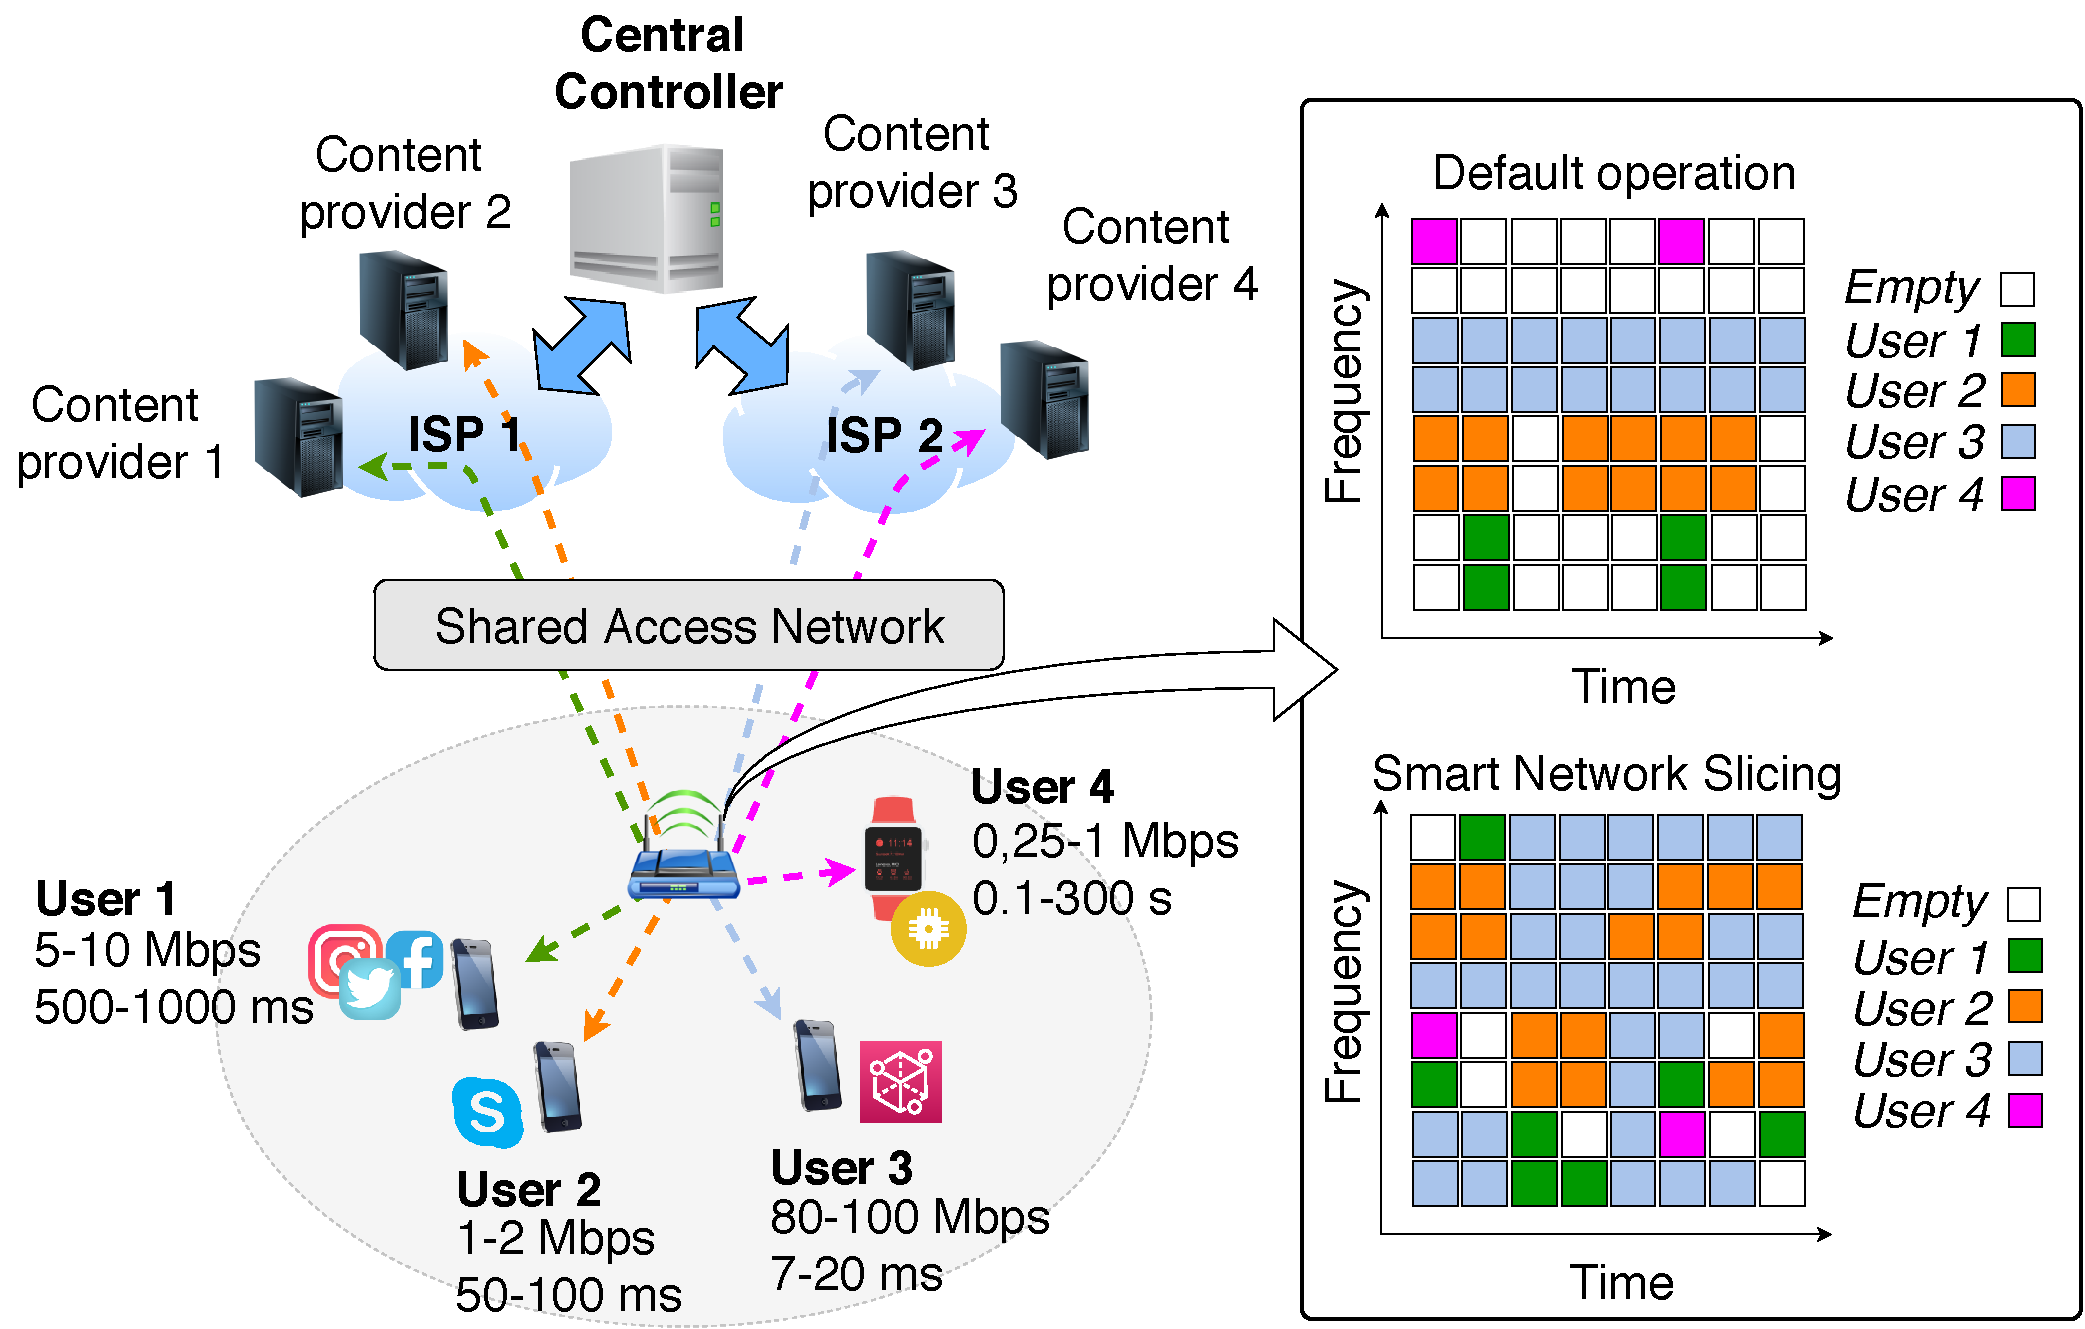
\includegraphics[width=1\columnwidth]{network_slicing_ofdma}\label{fig:network_slicing_ofdma}}
	\subfigure[Access Point association]{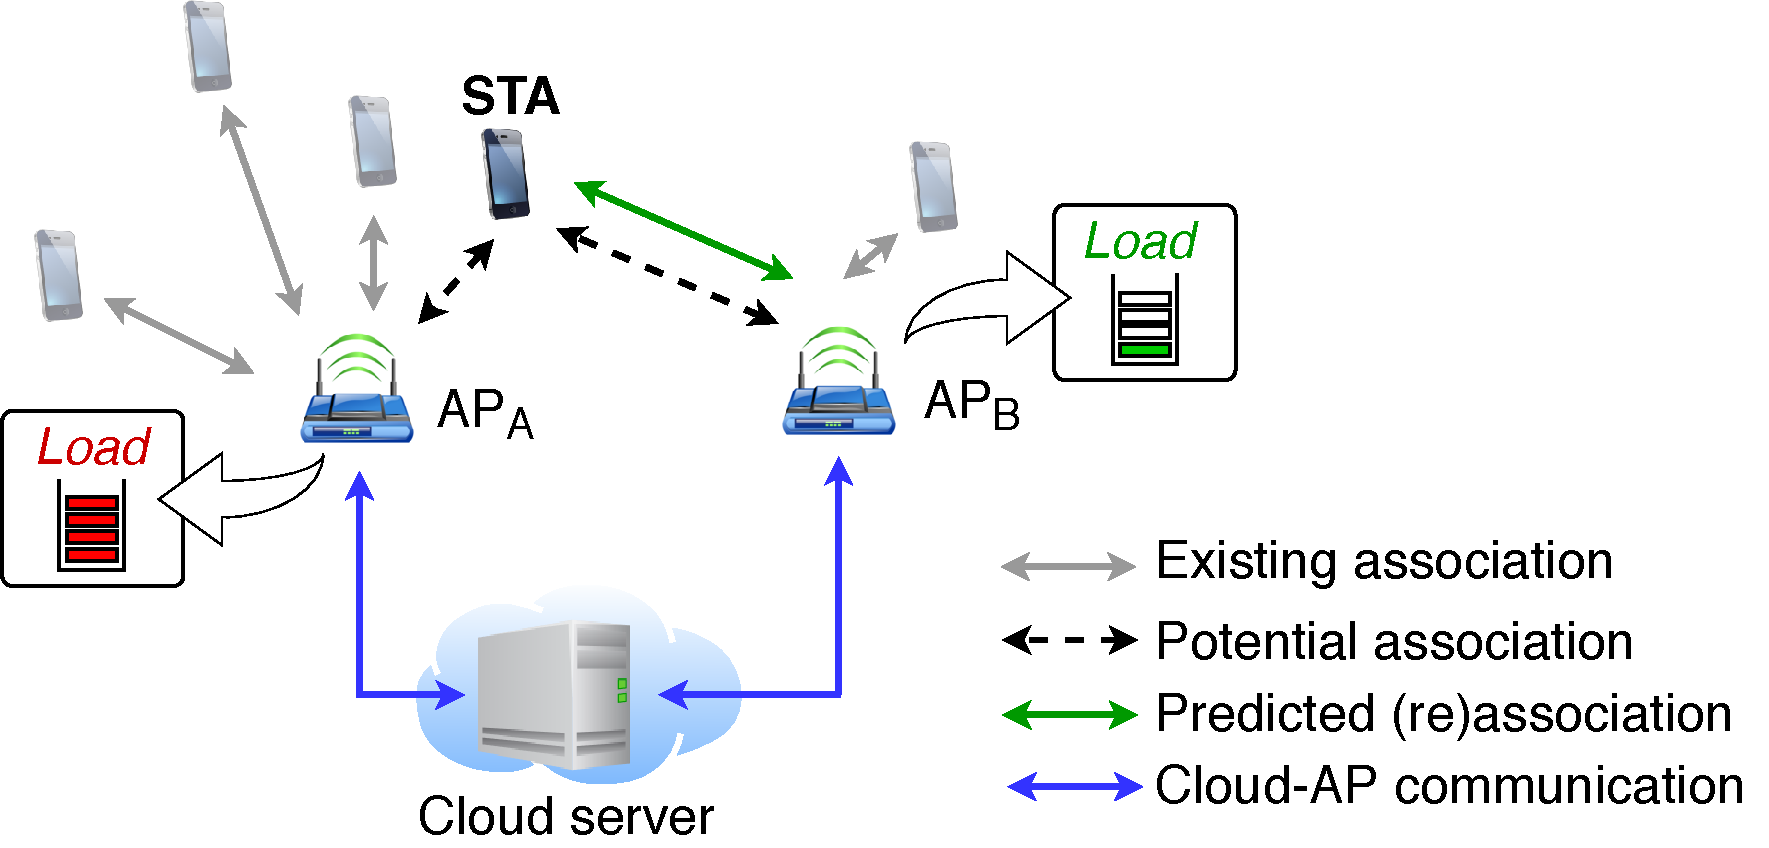
\includegraphics[width=1\columnwidth]{use_case_ap_association}\label{fig:use_case_ap_association}}
	\caption{Use cases of ML-based operation in WLANs. (a) OFDMA-based smart network slicing, (b) Cloud-oriented Access Point association.}
	\label{fig:use_cases}
\end{figure}

\subsubsection{OFDMA-Based Smart Network Slicing} 
Network slicing is one of the hottest topics in 5G because it allows separating network resources virtually to meet diverse application requirements. In next-generation WLANs, network slicing can be realized through the allocation of radio resources via orthogonal frequency-division multiple access (OFDMA). However, the heterogeneity of applications running in multiple devices and their subsequent elasticity prevent to assign frequency resources easily. 

The application of ML can overcome the aforementioned challenges by making predictions on the user requirements so that the access network can be optimized. As an example, Fig. \ref{fig:network_slicing_ofdma} shows a scenario where multiple users have different requirements, based on the applications they use. While the central controller can make predictions on user behavior, the local schedulers can consider information such as the user profile, the current performance, and the environmental circumstances. In this regard, the Access Point (AP) can allocate the most suitable OFDMA resources to each device, according to its predicted needs and current status of the network.

\subsubsection{Cloud-Based User Association and Handover}
Most of the current user association and handover procedures held in WLANs typically rely on strongest signal first (SSF) mechanisms. This might be problematic in terms of load balancing, thus potentially leading to severe performance degradation at saturated APs. By introducing ML, it is possible to handle contextual information such as the traffic load at the APs, which can support decision-making. Furthermore, mobility pattern prediction and predicted user requirements can be included in the system, thus empowering the association and handover mechanisms with insightful information. %\textcolor{orange}{Predictions can be provided, for instance, by Deep Neural Networks (DNN).}

The ML-enabled user association solution is illustrated in Fig. \ref{fig:use_case_ap_association}. A cloud-oriented service obtains data from the different connected WLANs (e.g., number of associated devices, traffic load, performance reports, etc.), which are used for training. Then, new requests are addressed by the ML mechanism, which chooses the best predicted AP for the (re)association, based on the corresponding optimization goals.

\subsubsection{Inference-Based Coordinated Scheduling}

Contrary to traditional cellular-type networks, WLAN deployments can be chaotic, especially in residential scenarios where anyone can set-up an AP and create a wireless network. This typically leads to scenarios with complex interactions among different Basic Service Sets (BSSs), which prevent the existing scheduling approaches to ensuring proper quality of service (QoS). Nevertheless, ML can be used to infer these interactions and provide a solution accordingly. In particular, through coordinated ML-assisted scheduling, different APs can trigger uplink/downlink transmissions from/to the appropriate stations (STAs), thus increasing the network throughput and reducing the number of packet collisions.

\subsubsection{Reinforcement Learning-Based Spatial Reuse} 
In contrast to centralized and cooperative ML approaches, local optimization is required for independent WLANs. In this regard, Spatial Reuse (SR) aims to improve channel utilization by means of sensitivity adjustment mechanisms. However, selecting the best sensitivity threshold is not trivial, given the complex spatial interactions that occur among WLANs and the high action space. With this purpose, RL can be introduced to improve spectral efficiency in a decentralized manner, so that each WLAN learns based on experience.

% ----------------------------------
% -
% 	-- ITU-T ARCHITECTURE --
% -
% ----------------------------------

\section{ITU Unified Architecure for Future Networks}
\label{section:itu_architecture}

\begin{figure*}[!ht]
	\centering
	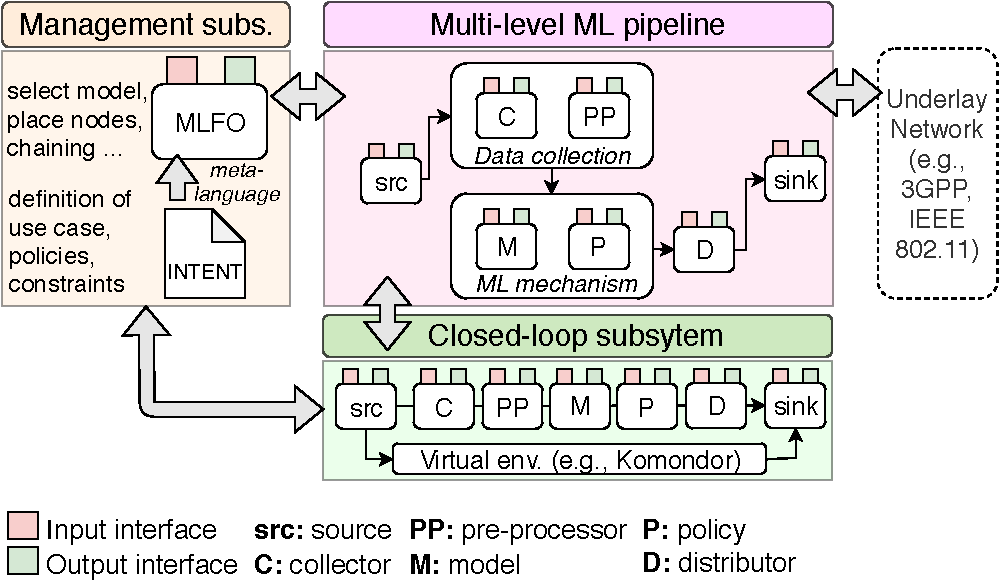
\includegraphics[width=0.6\textwidth]{itu_ml_architecture}
	\caption{ITU logical architecture for future networks \cite{itu2019architecture}.}
	\label{fig:itu_ml_architecture}
\end{figure*}

The FG-ML5G was created in November 2017 by its parent group, the ITU-T Study Group 13, with the aim of studying the integration of ML mechanisms into future networks. This includes the definition of interfaces, protocols, data formats, and architectures. During its lifetime, the FG-ML5G has released several reports and contributions. Among them, we highlight the ITU's logical interoperable architecture for future networks \cite{itu2019architecture}, which defines an ML overlay that operates on the top of any unspecified underlay network technology (e.g., 3GPP, EdgeX, IEEE 802.11). The ITU's architecture aims to fulfill a set of technology-agnostic high-level requirements by the utilization of ML. For instance, the architecture must be able to support multiple types of data, thus taking advantage of heterogeneous data sources. 

Figure \ref{fig:itu_ml_architecture} shows the elements that compose the ML overlay (management subsystem, multi-level ML Pipeline, and closed-loop subsystem), which are further described in the following subsections. Based on this overlay, ML applications can be instantiated in the logical entities (represented by white boxes), which are managed in a standard manner. %Communication among entities is done through input and output interfaces.

\subsection{Management Subsystem} 
The management subsystem is in charge of the deployment and the orchestration of the ML services so that they can operate in the underlying network. To that purpose, the Machine Learning Function Orchestrator (MLFO) entity is defined. The MLFO is first instantiated by an intent, which is a declarative mechanism that provides details on the ML use case to be applied. The ML intent, therefore, defines the methods and policies to be applied throughout the network and instantiates the elements of the multi-level ML Pipeline in the corresponding devices. In particular, the intent can use a meta language to define the policies and constraints that characterize the use case.

\subsection{Multi-Level Machine Learning Pipeline} 
The multi-level ML Pipeline is formed by a set of logical entities that perform the actual ML activity in a given network underlay. The ML Pipeline is instantiated and managed by the management subsystem and it is mainly in charge of the data collection and pre-processing, ML model application, and output distribution. The logical entities that compose the ML Pipeline are as follows:
\begin{itemize}
    \item \textbf{Source (src):} element that generates data to be used by the ML mechanism.
    \item \textbf{Collector (C):} element responsible for collecting the data generated by source nodes.
    \item \textbf{Pre-processor (PP):} element that prepares the data collected by the collector for its utilization by the ML mechanism.
    \item \textbf{Model (M):} ML model that is applied according to the use case.
    \item \textbf{Policy (P):} provides a set of constraints and/or guidelines that delimit the behavior of the model.
    \item \textbf{Distributor (D):} element that spreads the ML output across all the corresponding targets (or sinks).
    \item \textbf{Sink (sink):} target of the ML output that is allocated by the distributor.
\end{itemize}

\subsection{Closed-loop Subsystem} 
In order to address network dynamics, the ML operation is assisted by a closed-loop subsystem. In particular, a sandbox environment can be used to reproduce (internal network) or simulate (simulator/emulator) the effect of certain ML optimization, so that additional information is provided to the system beforehand. As for the ML Pipeline, the closed-loop subsystem is orchestrated by the management subsystem. Network simulators (e.g., ns-3, Komondor \cite{barrachina2019komondor}) are examples of closed-loop subsystems, which can serve two purposes: \emph{i)} generate synthetic data to be used for training, and \emph{ii)} conducting a simulation for devising the potential of a given ML method to be applied afterward on the real network.

% ----------------------------------
% -
% 	-- ML Architecture --
% -
% ----------------------------------
\section{Machine Learning-Aware Architecture for IEEE 802.11 WLANs}
\label{section:wlans_architecture}

IEEE 802.11 WLANs are versatile in the sense that many different kinds of deployments can be realized. Roughly, we differentiate between two main types:
\begin{itemize}
    \item \textbf{Enterprise:} a set of WLANs can be jointly operated from the edge and/or the cloud, thus providing management and orchestration functionalities (e.g., centralized authentication, channel allocation). Enterprise-like deployments are realized through extended service sets (ESS) and can be typically found in environments controlled by a single network operator, such as university campuses, offices, stadiums, etc. 
    \item \textbf{Residential:} each WLAN is responsible for its own management and operation. In the context of residential scenarios (but not limited to), ad-hoc WLANs such as personal hotspots are gaining popularity for infrastructureless communications (i.e., peer-to-peer). Ad-hoc WLANs are realized through the independent basic service set (IBSS).
\end{itemize}

Figure \ref{fig:overview_learning_approaches} illustrates the enterprise and residential-like deployments, as well as a set of IEEE 802.11 mechanisms (summarized in Table \ref{tab:opportunities_amendments}) that can potentially enable the utilization of ML in WLANs. These mechanisms can be used for data collection, training, and output distribution. By taking advantage of the current IEEE 802.11 mechanisms, ML can be introduced to WLANs in a non-intrusive manner, thus facilitating its immediate adoption. 

\begin{figure}[ht!]
	\centering
	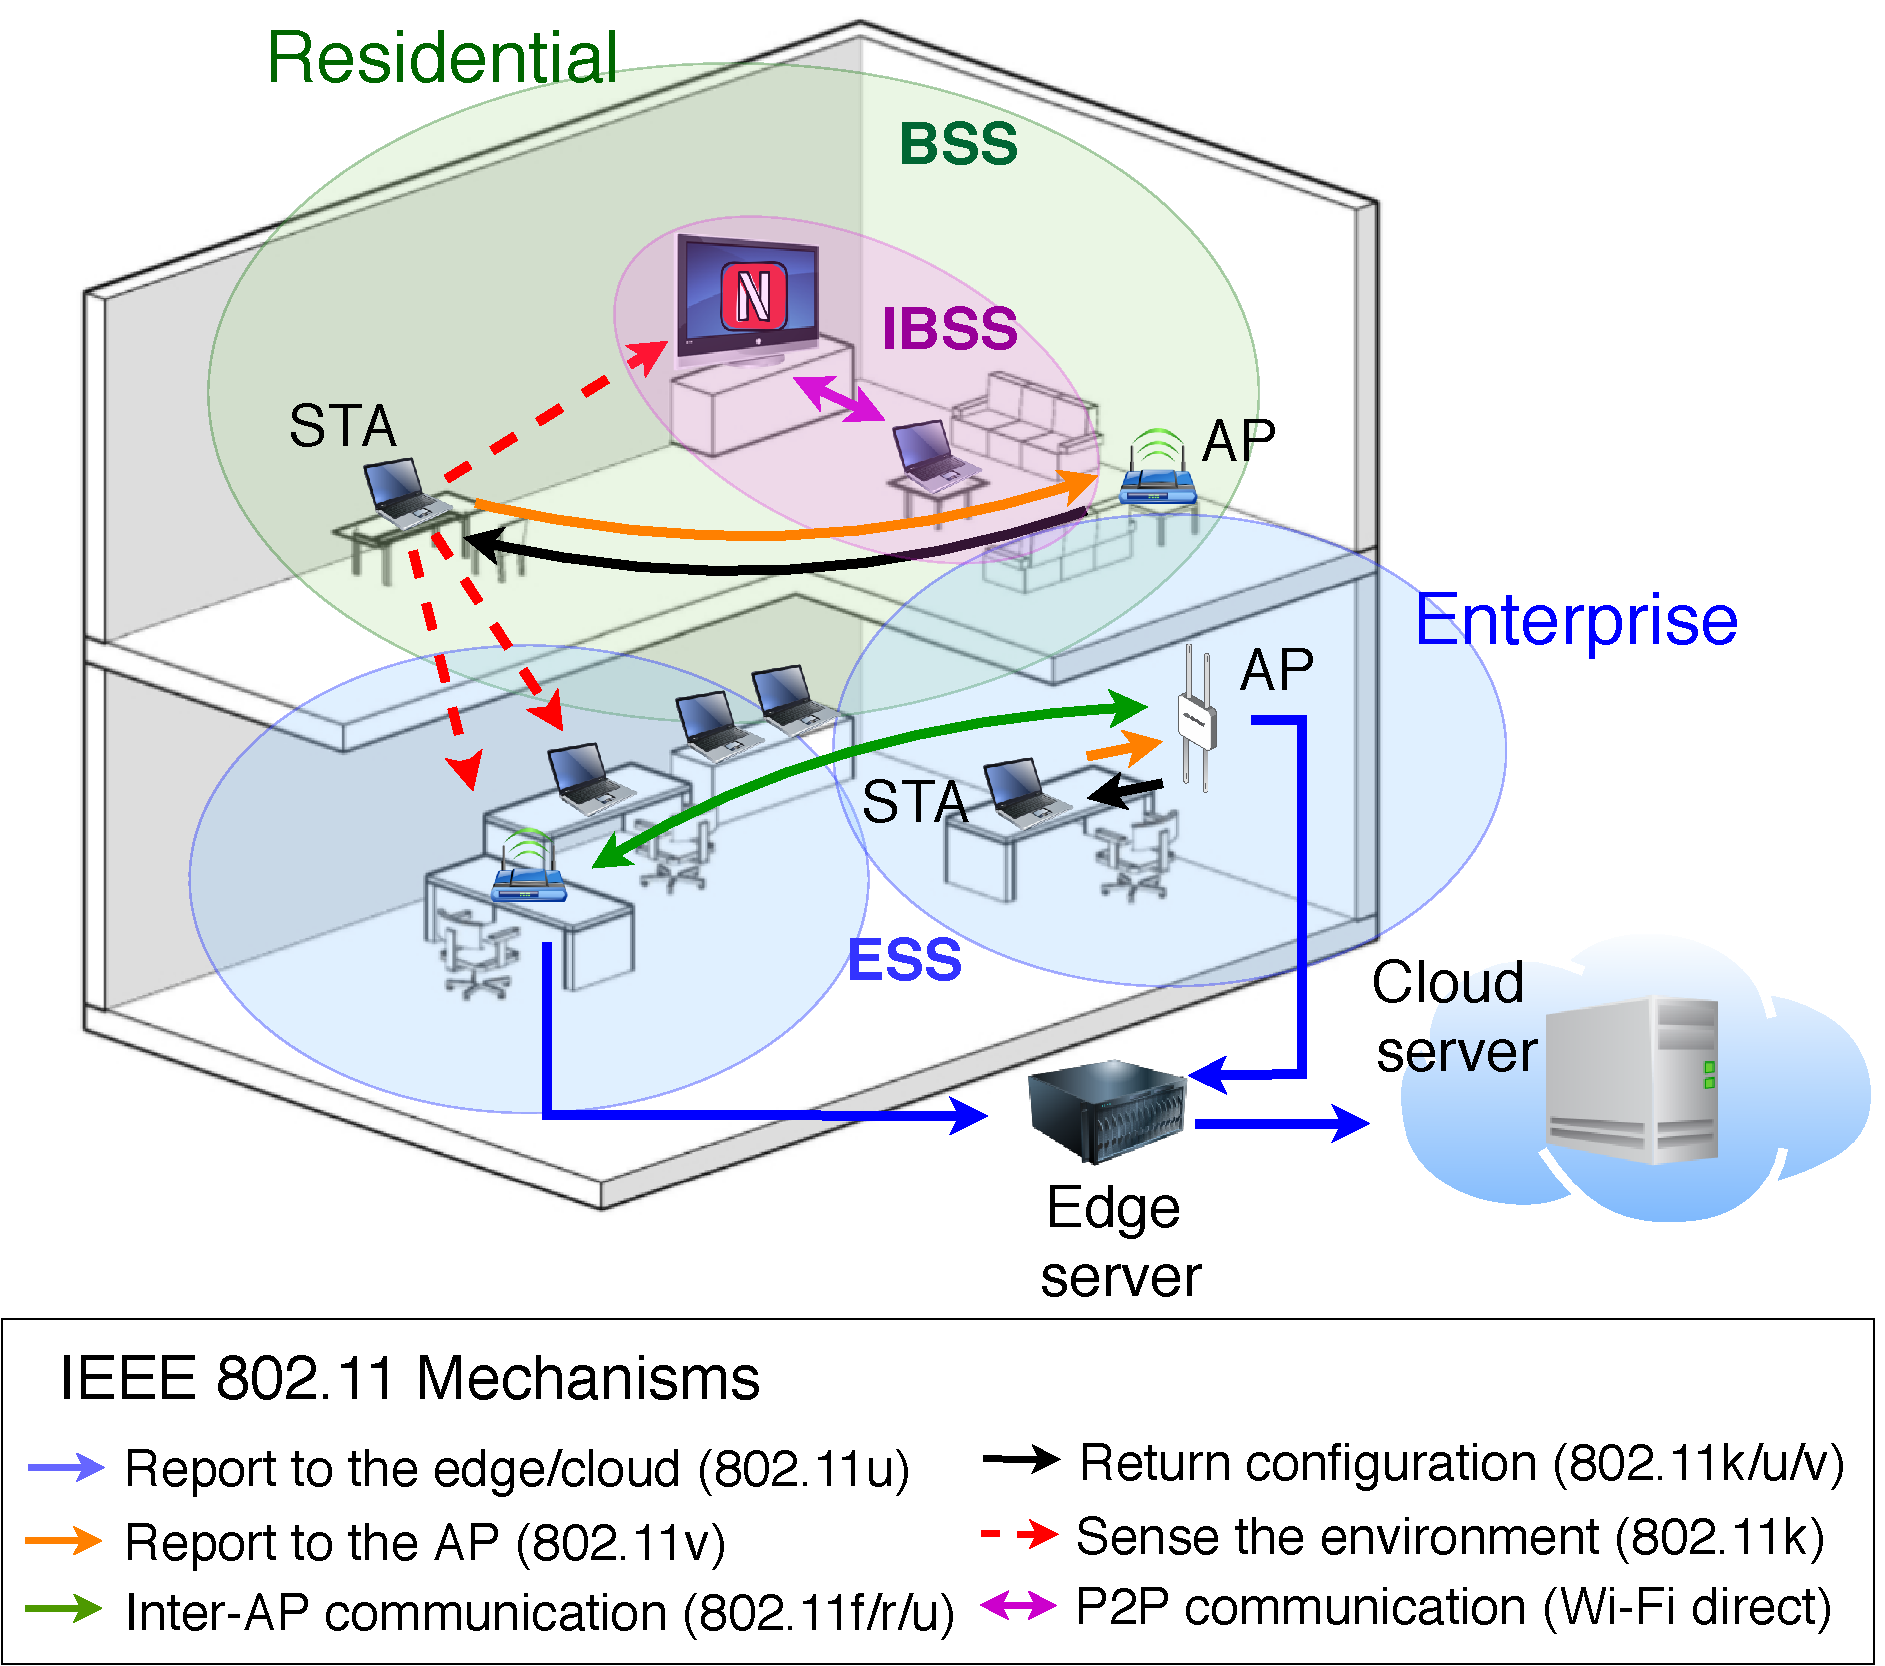
\includegraphics[width=\columnwidth]{overview_learning_approaches}
	\caption{Enterprise and residential-like deployments and complementary mechanisms from IEEE 802.11 amendments to enable the utilization of ML.}
	\label{fig:overview_learning_approaches}
\end{figure}

\begin{table*}[t!]
\caption{Features supported by 802.11 amendments that can enable the introduction of ML methods to WLANs.}
\label{tab:opportunities_amendments}
\centering
\begin{tabular}{|p{.12\textwidth}|p{.12\textwidth}|p{.7\textwidth}|}
\hline
\textbf{Feature} & \textbf{Amendments} & \textbf{Opportunities for ML application} \\\hline
Information gathering & 802.11k/r/v & A given ML mechanism can use information about the network topology or RF measurements to infer the behavior of other devices or to extract important environmental characteristics.\\\hline
Interopera-blity & 802.11f/u & Interoperability with other networks can be used to perform coordinated operations (e.g., scheduling, resource allocation). Besides, inter-AP communication procedures can enable centralized/coordinated mechanisms (e.g., federated learning). \\\hline
Security & 802.11w & ML mechanisms can use management frames that are protected so that a higher level of security is granted.\\\hline
Validity & 802.11t & Performance evaluation in WLANs through test metrics can be of great utility to define optimization goals within the ML  operation.\\\hline
\end{tabular}
\end{table*}

%%% CHALLENGES IN IEEE 802.11 WLANs
\subsection{Challenges in IEEE 802.11 WLANs}
\label{section:ieee_80211_wlans}
The application of ML methods in WLANs is tightly tied to the technological challenges posed by these types of networks. The major challenges encountered in wireless communications stand for fast data expiry and lack of resources for data handling (e.g., storage, computation, information exchange). In particular, IEEE 802.11 WLANs present the following challenges:
\begin{enumerate}
    \item \textbf{Network dynamics:} channel fluctuations (e.g., due to multipath fading), users mobility and varying traffic needs entail a big challenge to ML applications. As a result of network dynamics, ML methods need to constantly adapt to the environment, which may be achieved through continuous re-training.
    \item \textbf{Limited communication resources:} since Wi-Fi operates under unlicensed bands, resources are scarce and shared. Thus, any potential communication required by a certain ML mechanism (as for distributed learning) may fail or be delayed if the medium is congested. As a result, the ML operation must be robust and resilient enough in order to react to potential communication issues.
    \item \textbf{Limited computation and storage resources:} computation and storage resources may also be limited in WLANs, especially in residential-like deployments. Therefore, the ML operation should include computation-efficient procedures. Another implication of limited resources lies in the availability of information to be used by ML algorithms, especially for online learning methods.
    \item \textbf{Adversarial environment:} in many cases, Wi-Fi deployments are chaotic in the sense that many overlapping WLANs coexist without any kind of cooperation (e.g., residential buildings). This is a particularly interesting challenge for ML operation, which may lead to adversarial settings where different agents compete for the same resources. Moreover, multi-vendor devices may implement different ML mechanisms that may lead to clashing interests.
    \item \textbf{Legacy devices:} in a similar way to the previous case, ML-empowered WLANs may coexist with other legacy networks that do not perform any intelligent operation. It is then required for ML methods to be aware of those legacy devices, so that unfairness situations are avoided.
\end{enumerate}

Apart from the aforementioned WLAN-specific challenges, other inter-domain issues should be considered. First, security is required since ML mechanisms store and/or exchange sensitive data that may be exposed. Besides, interoperability should be tackled to allow the deployment of ML solutions to different underlay networks. In this regard, the standardized ITU ML Pipeline stands up as a promising solution.

%%% REALIZATION OF THE ADOPTED ARCHITECTURE
\subsection{Realization of the ML-Aware Architecture for IEEE 802.11 WLANs}
The various types of WLAN deployments and their computation and communication capabilities are closely linked to the ML solutions that can be applied to them, which can be categorized into \emph{cloud} and \emph{edge-oriented}. 

Cloud-oriented ML applications are characterized by
bearing high computational and storage resources, thus allowing to collect various types of data from multiple sources and to provide global and long-term solutions. The major challenge for cloud-oriented methods lies in the management of data, which entails dealing with synchronization, availability, and heterogeneity issues.

In edge-oriented mechanisms, the ML operation is mainly ruled by edge devices (e.g., APs and/or STAs), which, contrary to the cloud approach, typically lack powerful computation and storage resources. In consequence, edge-oriented mechanisms may only allow using simple and light-weight computing ML algorithms. Nevertheless, edge servers can be placed for providing more powerful solutions in a timely manner. The edge-oriented approach is useful for real-time ML applications that manage local (and even highly-varying) information.

Besides cloud and edge-oriented settings, we may distinguish between methods based on cooperation or not, depending on the inter-entity communication degree. In cooperative approaches, nodes interact among them for the sake of conducting the learning operation in a joint manner (e.g., use a shared reward). With this aim, reliable and timely connections among learners are often required. In this regard, \cite{lin2017deep} showed the role of communications on speeding up a distributed training procedure over a set of nodes in a network. Alternatively, for the non-cooperative case, the learning operation may lead to adversarial settings, especially since WLANs share resources such as frequency channels.

%\begin{figure*}[ht!]
%	\centering
%	\subfigure[ML approaches]{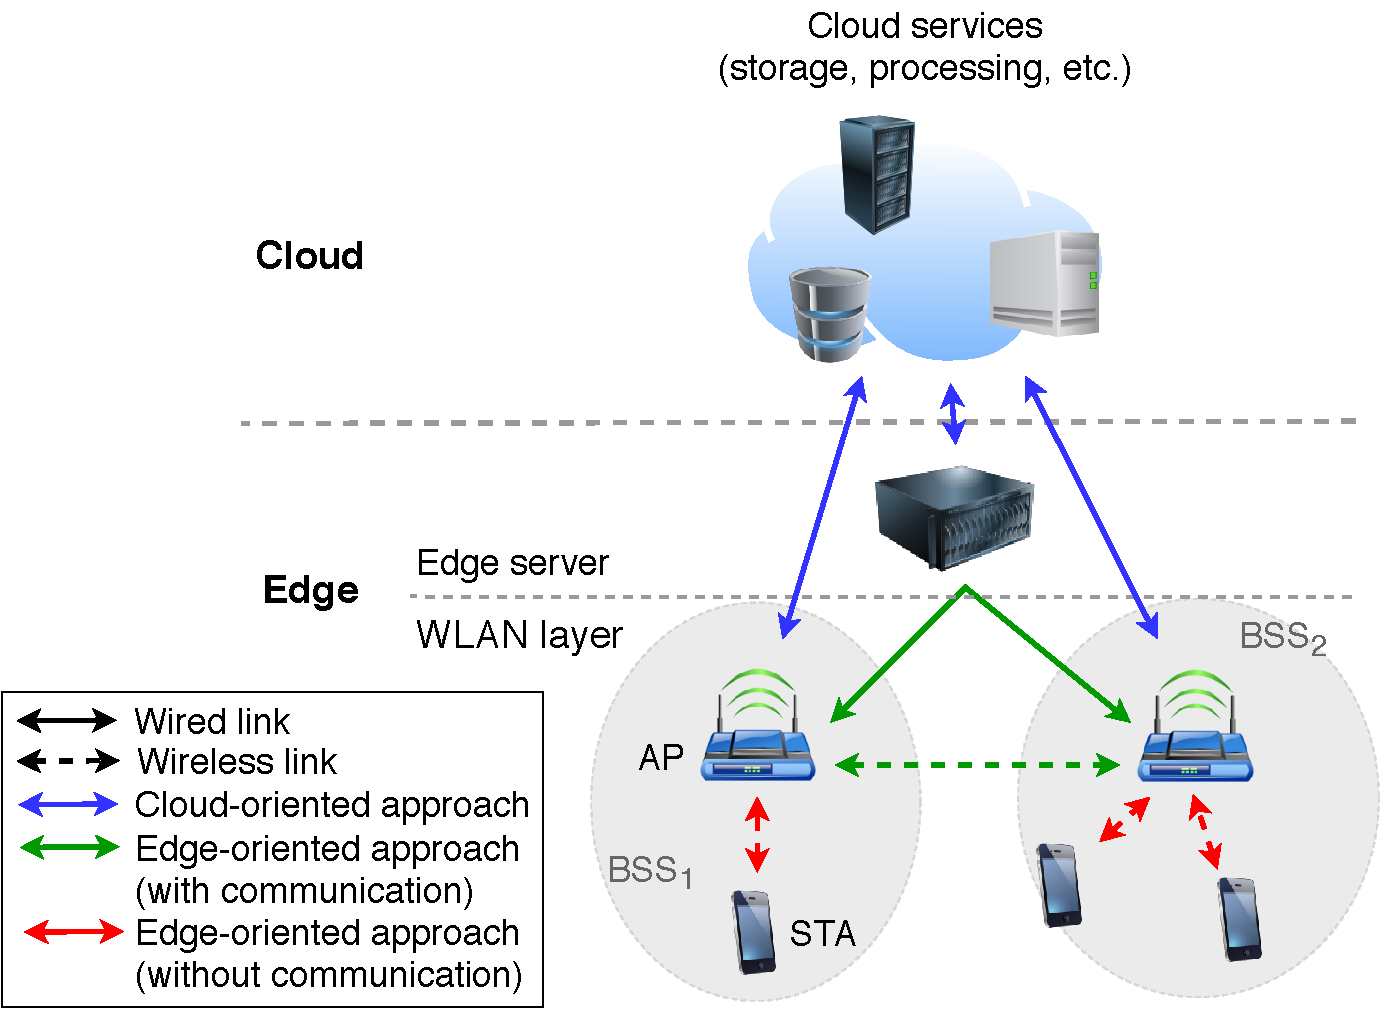
\includegraphics[width=1\columnwidth]{ml_architecture_wlan_1}\label{fig:ml_architecture_wlan_1}}
%	\subfigure[Realization of the ML pipeline]{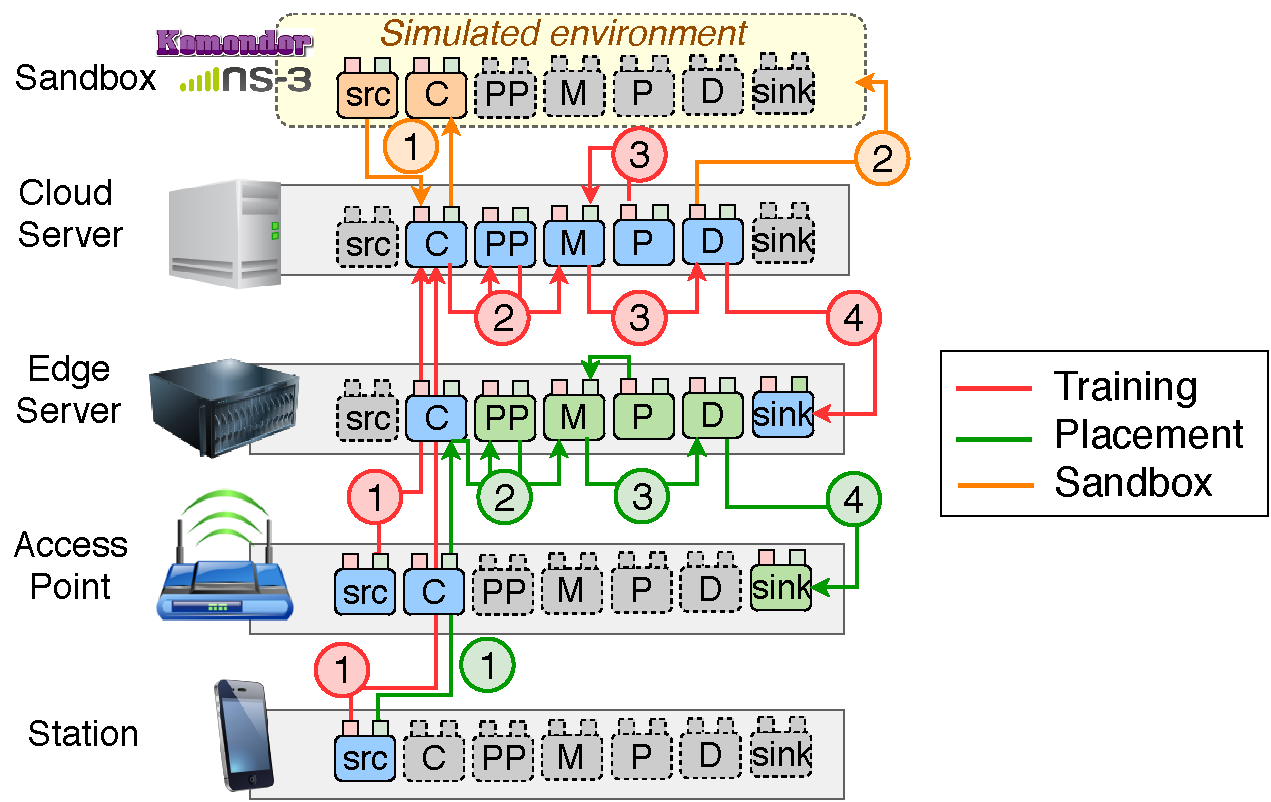
\includegraphics[width=1\columnwidth]{ml_architecture_wlan_2}\label{fig:ml_architecture_wlan_2}}
%	\caption{Realization of the ITU's ML architecture in IEEE 802.11 WLANs. (a) ML approaches based on the communication level and participating elements, (b) ML Pipeline realization of a hybrid ML-based solution for AP (re)association and handover.}
%	\label{fig:ml_architecture_wlan}
%\end{figure*}

\subsubsection{Example of the adoption of the architecture}
Through the adoption of the ITU's architecture, multiple entities in the ML Pipeline can be activated at different locations of the network, according to the selected learning approach. This expands the concept of cloud and edge computing and leads to hybrid solutions.% (e.g., combining centralized channel allocation with decentralized spatial reuse). 

In order to illustrate this (see Fig. \ref{fig:ml_architecture_wlan}), let us go back to the AP (re)association and handover example. We now consider a hybrid solution in which two main ML-oriented processes are held: training (learn from data) and placement (apply the learned knowledge). While the training procedure is carried out at the cloud (collect a lot of data from multiple sources), the placement operation is done at the edge (provide timely responses to new cases). Note, as well, that the placement phase can also contribute to re-train the system in an online manner. % shows the elements in the ML Pipeline that participate in the aforementioned example. 

\begin{figure}[ht!]
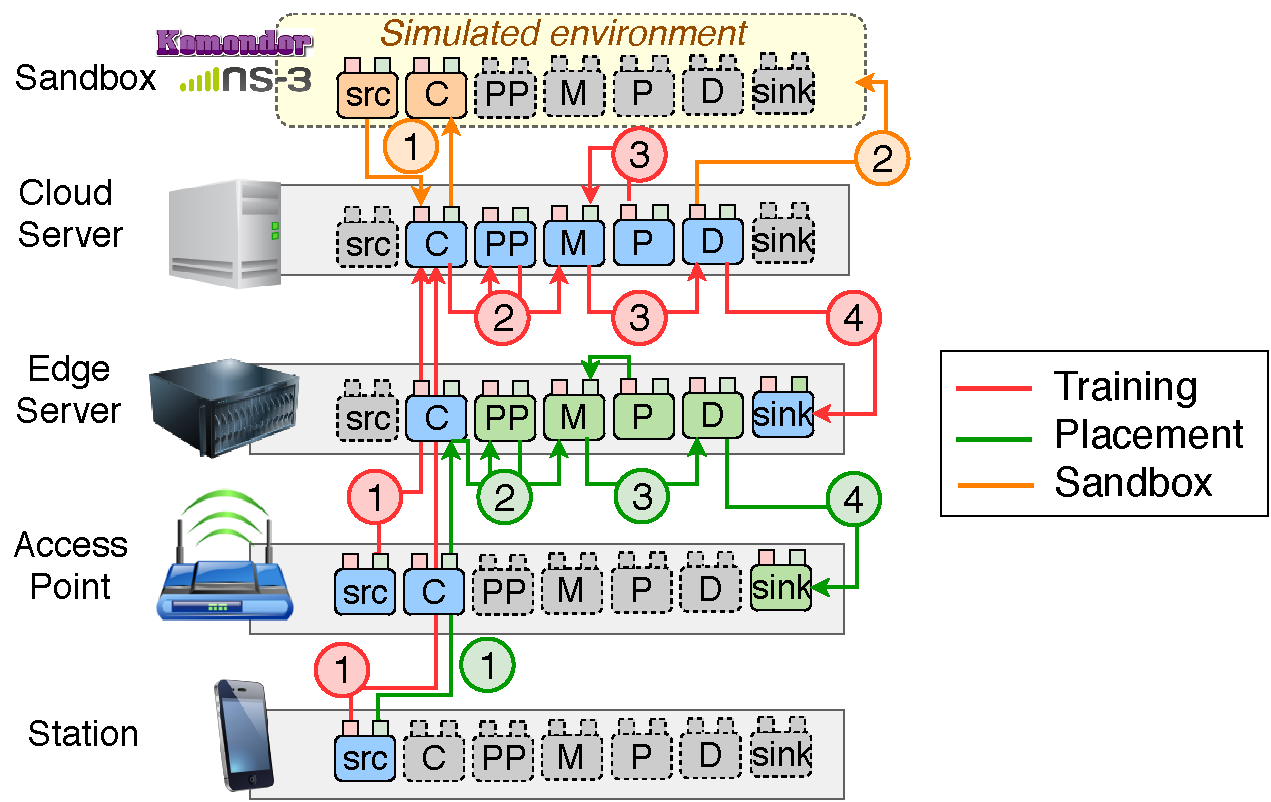
\includegraphics[width=1\columnwidth]{ml_architecture_wlan_2}
\caption{Realization of the ITU's ML architecture for IEEE 802.11 WLANs through a hybrid ML-based solution for AP (re)association and handover.}
\label{fig:ml_architecture_wlan}
\end{figure}

Specifically, the training procedure consists of the following steps (shown by red bullets in Fig. \ref{fig:ml_architecture_wlan}):
\begin{enumerate}
    \item \textbf{Data collection:} information of different nature is collected at the edge server from either APs and STAs. Edge nodes provide contextual data such as user information (e.g., current location), performance (e.g., throughput, delay), application data (e.g., traffic load), or channel status reports (e.g., the power received from interfering nodes). This information is then used either for training or for feeding auxiliary algorithms (e.g., predict user behavior) that help the main AP association procedure.
    \item \textbf{ML input preparation:} the data collected at the cloud is prepared by the pre-processor so that the ML method can properly manage it. For instance, in case of applying a multiple linear regression, the input user information needs to be converted into normalized features (e.g., convert the throughput given in Mbps into a scalar between 0 and 1).
    \item \textbf{ML method application:} on applying the ML method, policies are also taken into account for generating the final output result. In this case, a given AP may have specific constraints regarding its occupation or the maximum number of associated STAs. The policies are strongly tied to the capabilities of the devices or the existing regulations (e.g., frequency channels available due to antenna capabilities, maximum regulated transmission power).
    \item \textbf{Output distribution:} once the ML method generates the output (i.e., the predicted function for new (re)associations), it is distributed throughout the sink edge servers, which are then prepared to give quick response to new cases.
\end{enumerate}

When it comes to placement phase, we find the following operations (shown by green bullets in Fig. \ref{fig:ml_architecture_wlan}):
\begin{enumerate}
    \item \textbf{Handle new cases:} new (re)association requests or potential handovers are detected based on newly acquired information from STAs. This information is collected by the edge server.
    \item \textbf{Pre-processing:} the acquired information is then processed by the edge server, as for the training phase.
    \item \textbf{Run the ML solution:} the ML method provided by the cloud is applied locally at the edge server, which provides an output for the new placement case.
    \item \textbf{Apply the ML solution:} finally, the output solution to new (re)association cases is distributed to the corresponding sinks.
\end{enumerate}

Finally, it is worth pointing out the role of the sandbox (e.g., a simulated environment), which can be mainly twofold (shown by orange bullets in Fig. \ref{fig:ml_architecture_wlan}):
\begin{enumerate}
    \item \textbf{Generate data for training:} the sandbox can act as a source in the ML Pipeline by generating synthetic data for training purposes. Notice that the data provided by the sandbox is limited to several factors (e.g., accuracy of the simulation model, similarity of the sandbox to the real environment). Also, data collected from the network can be used in the sandbox.
    \item \textbf{Preliminary model testing:} alternatively, the sandbox can serve to test and validate the output of the ML method (e.g., test a solution before being applied to the real network).
\end{enumerate}

% ----------------------------------
% -
% 	-- Conclusions --
% -
% ----------------------------------
\section{Concluding Remarks}
In order to sustain progress in wireless networks, it is needed to accommodate the operation of ML as an intrinsic part of communications. Nevertheless, current networks are not yet prepared for the pervasive adoption of ML-based operation. Hence, disruptive architectural changes are required. For the sake of moving forward in this field, this article introduced the ITU's unified architecture for future networks and provided a realization for IEEE 802.11 WLANs. The different forms of Wi-Fi networks allow uplifting the flexibility characteristic of the ITU's architecture, thus empowering from edge to cloud-oriented approaches, including hybrid approaches.

To conclude, future wireless networks are envisioned to share a common flexible architecture that allows a fast adaptation of resources to accommodate a plethora of ML-enabled network verticals. Nevertheless, a lot of effort is still required before reaching fully intelligent wireless networks. Among several open issues, we highlight the ones related to data handling (\textit{how and where to store data? how to assess the expiry of data?}), orchestration (\textit{how would several ML approaches would behave in conjunction? how to distribute the ML operation? how to deal with heterogeneity?}), and robustness of the ML methods (\textit{how to deal with uncertainty? how to prevent network failures?}). 

% -------------------------------------
% Acknowledgment
%
% -------------------------------------
\section*{Acknowledgments}  
This work has been partially supported by grants MDM-2015-0502, 2017-SGR-11888, by WINDMAL PGC2018-099959-B-I00 (MCIU/AEI/FEDER,UE), by a Gift from the Cisco University Research Program (CG\#890107) Fund, and by SPOTS project (RTI2018-095438-A-I00) funded by the Spanish Ministry of Science, Innovation and Universities. The work by Sergio Barrachina-Mu\~noz is supported by an FI grant from Generalitat de Catalunya.

% -------------------------------------
% Bibliography
%
% -------------------------------------

\bibliographystyle{unsrt}
\bibliography{bibliography}

% -------------------------------------
% Biographies
%
% -------------------------------------
\section*{Biographies}

\begin{description}
	\item[Francesc Wilhelmi] (francisco.wilhelmi@upf.edu) holds a B.Sc. degree in Telematics Engineering (2015) and an M.Sc. in Intelligent and Interactive Systems (2016), both from Universitat Pompeu Fabra (UPF). He is currently pursuing a Ph.D. in Information and Communication Technologies at UPF.
	%
	\item[Sergio Barrachina-Mu\~noz] (sergio.barrachina@upf.edu) obtained his B.Sc. degree in Telematics Engineering and his M.Sc. in Intelligent Interactive Systems in 2015 and 2016, respectively, both from Universitat Pompeu Fabra (UPF), Barcelona. Currently, he is a PhD student and teacher assistant in the Wireless Networking research group at UPF.% His main research interests are focused on developing autonomous learning methods and techniques for improving the performance of next-generation wireless networks.
	%
	\item[Boris Bellalta] (boris.bellalta@upf.edu) is an Associate Professor in the Department of Information and Communication Technologies (DTIC) at Universitat Pompeu Fabra (UPF). He is the head of the Wireless Networking research group at DTIC/UPF.% His research interests are in the area of wireless networks, with emphasis on the design and performance evaluation of new architectures and protocols.
	%
	\item[Anders Jonsson] (anders.jonsson@upf.edu) is the director of the Artificial Intelligence and Machine Learning group at Universitat Pompeu Fabra (UPF). He received his Ph.D. in computer science in 2005 from the University of Massachusetts Amherst, USA, and has been at UPF ever since. %Anders' main research focus is sequential decision making, formulated both as AI planning and as reinforcement learning, but he also conducts research in other areas of AI and machine learning. %He is interested in many extensions of the problem of sequential decision making, such as regularization and exploration, hierarchical representations of decision strategies, problems involving multiple agents, and adapting existing techniques to lifelong learning, allowing a system to learn and explore during extended periods of time.
	%
	\item[Cristina Cano] (ccanobs@uoc.edu) holds a Ph.D. (2011) in Information, Communication and Audiovisual Media Technologies from Universitat Pompeu Fabra (UPF). She has been a research fellow in the Hamilton Institute of the National University of Ireland, Maynooth (2012-2014), in Trinity College Dublin (2015-2016) and in Inria-Lille in France (first half of 2016). Currently, she is an associate professor at Universitat Oberta de Catalunya (UOC). %Her research interests include coexistence of wireless heterogeneous networks, distributed resource allocation and online optimisation. %
	\item[Vishnu Ram] (vishnu.n@ieee.org) worked for Motorola/Nokia/Siemens in advanced technologies teams for 21 years. He was a Scientific Advisory Board Associate (SABA) member of Motorola Networks. He has published several drafts in IETF, contributed to ETSI, 3GPP in his role as a senior specialist (Radio Resource Management). He is currently working as an Independent Researcher. %He holds 12 International Granted Patents (and several pending applications) and has several publications. 
	
\end{description}

\end{document}